\documentclass[conference]{IEEEtran}
\IEEEoverridecommandlockouts
\usepackage{cite}
\usepackage{amsmath,amssymb,amsfonts}
\usepackage{algorithmic}
\usepackage{graphicx}
\usepackage{textcomp}
\usepackage{xcolor}
\usepackage{booktabs}
\def\BibTeX{{\rm B\kern-.05em{\sc i\kern-.025em b}\kern-.08em
    T\kern-.1667em\lower.7ex\hbox{E}\kern-.125emX}}
\begin{document}

\title{AI-Powered Liver Disease Prediction Using Random Forest and Kolmogorov–Arnold Networks (KAN)}\\

\author{
\IEEEauthorblockN{
    \begin{tabular}{ccc}
        % ===== Author 1 =====
        \begin{minipage}[t]{0.28\textwidth}
            \centering
            \textbf{Dr.P.J.Beslin Pajila \textsuperscript{1}}\\[2pt]
            \textit{Department of Computer Science and Engineering,}\\
            \textit{Vel Tech Rangarajan Dr. Sagunthala R\&D Institute of Science and Technology,}\\
            Avadi, Chennai, India.\\
            beslin.kits@gmail.com 
        \end{minipage}
        &
        % ===== Author 2 =====
        \begin{minipage}[t]{0.28\textwidth}
            \centering
            \textbf{Arjun Kumar\textsuperscript{2}}\\[2pt]
            \textit{Department of Computer Science and Engineering,}\\
            \textit{Vel Tech Rangarajan Dr. Sagunthala R\&D Institute of Science and Technology,}\\
            Avadi, Chennai, India.\\
            vtu21343@veltech.edu.in
        \end{minipage}
        &
        % ===== Author 3 =====
        \begin{minipage}[t]{0.28\textwidth}
            \centering
            \textbf{Shivam Kumar\textsuperscript{3}}\\[2pt]
            \textit{Department of Computer Science and Engineering,}\\
            \textit{Vel Tech Rangarajan Dr. Sagunthala R\&D Institute of Science and Technology,}\\
            Avadi, Chennai, India.\\
            vtu21339@veltech.edu.in
        \end{minipage}
    \end{tabular}
}
}
\maketitle


\begin{abstract}
liver disease is a significant health issue of the global society, claimed to result in more than two million deaths annually in the world. It is important that the disease be diagnosed early to be treated successfully and the current means of diagnosing the illness have several shortcomings; they are slow, rely on the judgment of the doctor and may not be easily available in rural regions. This is a work where we developed a machine learning system to predict liver disease out of standard blood test samples. We compared 1,583 Indian Liver Patient Dataset and other medical databases on patients and examined ten clinical measures such as age, gender, bilirubin level, liver enzymes, and protein levels. We have tested five machine learning models, such as Logistic Regression, Random Forest, XGBoost, Multi-Layer Perceptron, and KolmogorovArnold Networks. Random Forest was the most overall accurate with 90.76 percent, 89.87 percent, 95.23 percent and 95.45 percent accuracy, precision, recall and ROC-AUC respectively. KAN achieved the greatest ROC -AUC of 95.57 percent but it is also much more interpretable as it has learnable spline transformations. We have analyzed that total bilirubin, alkaline phosphatase, and AST are the most significant characteristics to be considered in prediction. Our project is a web application based on FastAPI and React that provides immediate risk assessment in three categories: Low, Moderate, and High. This article demonstrates that machine learning has the potential to assist physicians in screening liver disease more efficiently and effectively, which may allow identifying cases early and providing better treatment to patients.
\end{abstract}

\begin{IEEEkeywords}
Index Terms Liver Disease, Machine Learning, Random Forest, KolmogorovArnold Network, Clinical Decision Support, Medical AI, Explainable.
\end{IEEEkeywords}

\section{Introduction}
The problems of liver diseases are enormous, encompassing viral hepatitis, alcoholic liver disease, NAFLD, cirrhosis and liver cancer. According to the WHO, these conditions claim approximately 2 million lives every year, which is a margin of 4 percent of all deaths in the world annually \cite{topol2019}. The most common sore thing about liver disease is that they tend to manifest later when a lot of damage would have been caused. The initial issues are nearly silent hence the patients do not see any visible evidence until the disease has moved to the advanced stages where the remedies available become extremely scarce and the results become extremely dismal.

The classical method of liver diagnosis is a multi-phased, lengthy procedure that integrates the history of the patient, physical examination, lab tests, x-rays, and even biopsy. Blood tests of bilirubin, AST, ALT, alkaline phosphatase and proteins such as albumin provide doctors with important information \cite{ramana2011}. Nevertheless, the standard workflow has many disadvantages. To start with, it may take 24-48 hours to deliver lab results to the doc. Second, the interpretation greatly relies on the experience of the clinician, which causes inconsistent diagnoses, in particular, in the cases that are ambiguous. Third, urban clinics and specialists shortage in the countryside implies that diagnoses are not timely made or treatment is postponed. Lastly, in the majority of the conventional approaches, the answer is yes or no without any probability scores that would enable physicians and patients to choose more wisely.

It is clear that machine learning has presented some very interesting new opportunities in medical diagnosis and clinical decision making. Such algorithms are able to find complicated patterns in medical data which can be difficult to reveal by human specialists through automatic means only to be identified by these algorithms \cite{lecun2015, rajkomar2018}. In contrast to the computer systems controlled by rules, current ML models are trained on patient data and continue to enhance their prediction. Ensemble techniques such as the Random Forest are constructed based on a set of decision trees to provide more precise predictions than individual models do\cite{breiman2001}. Multi-processing layers have been shown to be used with deep learning techniques that can analyze medical images and classify diseases with impressive results \cite{esteva2017}.Deep-learning methods that use multiple processing layers have been demonstrated as making such claims and analyzing medical pictures in order to classify diseases with great results and accuracy Multi-processing layers have been shown to be used in deep-learning techniques in order to make such claims and analyze medical pictures in order to classify diseases with the great results and accuracy. Several studies show that the ML systems are able to be equal or even more accurate with respect to diagnoses of skilled physicians in different medical fields.

Despite these remarkable achievements, there is still a significant challenge to ubiquitous use of machine learning in healthcare, the so-called black box problem. The complexity of neural networks makes doctors difficult to comprehend the reasons a certain diagnosis was drawn, which undermines confidence in the environment where false predictions may cause severe consequences to patients \cite{ribeiro2016, lundberg2017}. This has prompted the development of interpretable models such as SHAP and LIME that attempt to understand model predictions. Nonetheless, these approaches are used once the decision is made and do not address the underlying issue of transparency of neural networks.

The fact that our research combines two approaches, which are complementary, addresses the issue of accuracy and interpretability \cite{liu2024}. Random Forest We train predictive models in KAN because it is more interpretable and Random Forest because it has a high-quality predictive performance and built-in feature importance. KAN uses spline curves, which are learnable to all the input features, unlike the traditional neural network which uses a single activation function on all the input features, which allows us to view how the model does precisely process individual values of blood tests. We have developed the two models as an easy-to-use web application, which provides immediate predictions with unambiguous levels of risk, and the system is now ready to implement it in any direction, whether a small clinic or a big hospital.

\section{Related Works}

Within the past ten years, machine learning to predict liver disease has been applied by a number of researchers and is getting more and more advanced over time. This was one of the first attempts to be done with the Indian Liver Patient Dataset (ILPD) \cite{ramana2011} where Naive Bayes, C4.5 decision trees, k-nearest neighbors and neural networks were tested. They discovered ensemble techniques reached an accuracy of 70.23\%  which was higher than any one model and was a good baseline to subsequent efforts. They also emphasized the importance of selecting the appropriate features and preprocessing the data in their study since the dataset is imbalanced and the majority of the patients already have the disease.

Ensemble learning is quite effective in medical prediction. Kumar et al. \cite{kumar2020}tested various approaches to ML to identify early-liver disease and demonstrated that a Random Forest may possess more than 83\% accuracy under the right conditions. Their study of the most significant features proved that bilirubin, albumin and alkaline phosphatase are good indicators and this is consistent with what is already known about liver functions by the doctors. Their findings indicate that tree-based ensemble algorithms are useful in automatically obtaining complicated associations among a number of blood-test markers without requiring manual feature engineering.

DNN can potentially learn sophisticated nonlinear trends in health data. One of the canonical textbooks on deep learning is Goodfellow et al. \cite{goodfellow2016} which discusses different architectures including Multi-layer perceptrons with dropout regularization that prevents overfitting when the data available is limited. There has been mixed success in applying these neural networks to classification of liver disease depending on the amount of data available, and the balance of the dataset. The greatest issue with the conventional neural networks in the medical field is that they are so-called black boxes, meaning their decision-making method is not visible to the physicians and thus it is difficult to place trust on them \cite{miotto2018}.

The other method that has been successful in medical prediction is gradient boosting. An effective implementation of the algorithm is XGBoost, developed by Chen and Guestrian \cite{chen2016} which builds the trees of the decision one after another in such a way that the new tree attempts to correct the errors of the preceding ones. It has been successful with numerous medical classification problems. An overview of literature on liver disease diagnosis identified that ensemble models such as the XGBoost and the Random Forest typically perform better than more basic models, and that their average accuracy is approximately 86\% \cite{sarker2021}. Nonetheless, issues with low quality of data, missing values, and the ability to transfer models to patients of other populations are only some of the problems that still need to be solved.


Due to the value of interpretability in the medical field, scientists have put a significant effort in creating explainable AI solutions. Lundberg and Lee \cite{lundberg2017} proposed SHAP (SHapley Additive exPlanations) as a method that involves the application of game theory concepts to determine the contribution of each feature to a prediction. The SHAP is able to explain individual predictions and remain consistent with the mechanism of action of the overall model, enabling doctors to realize what blood-test combinations resulted in a specific diagnosis. SHAP is currently used by a variety of medical AI systems but is an add-on tool, analyzing the model after making predictions instead of establishing interpretability as part of the model structure.

Recent research on neural network design has explored alternatives to traditional MLP architectures. Liu et al. \cite{liu2024} introduced Kolmogorov--Arnold Networks, which take a completely different approach by replacing fixed activation functions with learnable spline curves. Based on a mathematical theorem by Kolmogorov and Arnold, KAN breaks down complex functions into simpler one-dimensional transformations that can be visualized for each input feature. Early experiments showed that KAN performs as well as or better than MLPs while using 10$\times$ fewer parameters and being much more interpretable because you can actually see the learned splines—a big advantage for medical applications where doctors need to understand how the model works.

Transfer learning and domain adaptation have been investigated for improving model performance when training data is limited. Zhang et al. \cite{zhang2022} reviewed transfer learning applications in healthcare, showing that models can be adapted across different medical tasks and populations. While most transfer learning research focuses on medical imaging, recent work has begun exploring similar techniques for structured clinical data from electronic health records.

Modern deployment frameworks have made it feasible to serve machine learning models in clinical settings with minimal latency. Recent advances in web technologies and asynchronous Python frameworks enable real-time prediction systems that meet the strict performance requirements of clinical workflows \cite{rajkomar2018}. Such systems are able to support multiple users simultaneously and maintain sub-second response times through such techniques as model caching and efficient request processing.

The theoretical foundations of ensemble methods come from some important early research. Breiman \cite{breiman2001} created Random Forest and proved mathematically that ensembles work better when the individual trees are diverse (low correlation) but still accurate on their own. This insight helps us choose the right settings for things like sample size, how many features to use, and tree depth. Breiman also showed that Random Forest naturally tells you which features are important by measuring how much each one improves the predictions, so you don't need any extra tools to interpret the results.

\section{Existing System}

Current clinical practice for liver disease diagnosis begins when patients present with symptoms such as jaundice, hepatomegaly, ascites, or abnormal routine lab results. Physicians order comprehensive liver function panels including total and direct bilirubin, AST, ALT, alkaline phosphatase, GGT, total protein, albumin, globulin, and albumin-to-globulin ratio.

The conventional diagnostic workflow involves blood sample collection, laboratory processing using colorimetric or enzymatic assays, quality control verification, and result reporting through electronic health records. This process typically requires 24-48 hours, creating delays that may be critical for patients with acute liver decompensation or rapid-onset liver failure.

The existing system has several limitations: binary classification without probability scores, susceptibility to cognitive biases in interpretation, limited access to hepatology specialists in rural regions, lack of automated decision support for urgency assessment, and absence of systematic population screening protocols. These deficiencies result in delayed diagnoses, missed early-stage disease cases, and suboptimal resource allocation as chronic liver disease burden increases.

\section{Proposed System}
We developed a machine learning system that analyzes blood test results and provides immediate risk predictions. The system accepts standard clinical parameters and uses trained models to predict liver disease risk with confidence scores.

Five classification models were implemented: Logistic Regression (baseline), Random Forest (ensemble of decision trees), XGBoost (sequential ensemble correcting prior errors), Multi-Layer Perceptron (neural network with multiple hidden layers), and Kolmogorov-Arnold Network (interpretable architecture with learnable spline transformations).

All models were trained on 1,583 patient records from the Indian Liver Patient Dataset and other medical repositories. Input features include age, gender, total bilirubin, direct bilirubin, alkaline phosphatase, ALT, AST, total protein, albumin, and albumin-to-globulin ratio.

The system addresses critical limitations of conventional diagnostic workflows by providing instant risk stratification without requiring specialist expertise. Unlike traditional binary classification approaches, our system outputs probability scores and categorizes risk into interpretable levels (Low, Moderate, High), enabling clinicians to make informed decisions about patient management, follow-up schedules, and referral urgency. This probabilistic approach is particularly valuable in resource-limited settings where immediate access to hepatology specialists may not be available.

Random Forest achieved the highest accuracy with over 90% correct classification. KAN provides complementary interpretability by learning different transformation curves per feature rather than using a single activation function.

We deployed a web application with FastAPI backend and React + Material-UI frontend for clinical use.

\section{Architecture}

The system follows a client-server architecture with separation of concerns for maintenance and scalability.

The frontend is a React web application that runs in any browser and adapts to different screen sizes. Users enter patient blood test values through an interactive form.

The backend uses FastAPI and listens on port 8000 for incoming requests. It validates required information before processing predictions. The server applies preprocessing steps: converting gender to numerical values and normalizing blood test measurements using standardization (zero mean, unit variance).

The machine learning models are loaded into server memory at startup. Random Forest contains 200 decision trees with learned splitting rules, while KAN stores neural network weights including spline parameters.

The system converts probability outputs to classifications (disease present if > 0.5, absent if < 0.5) and risk categories: Low (0-0.25), Moderate (0.25-0.5), High (0.5-0.75), and Very High (0.75-1.0).

Fig.~\ref{fig:architecture} illustrates the data flow from user input through preprocessing and model inference to formatted predictions.

\begin{figure}[htbp]
\centerline{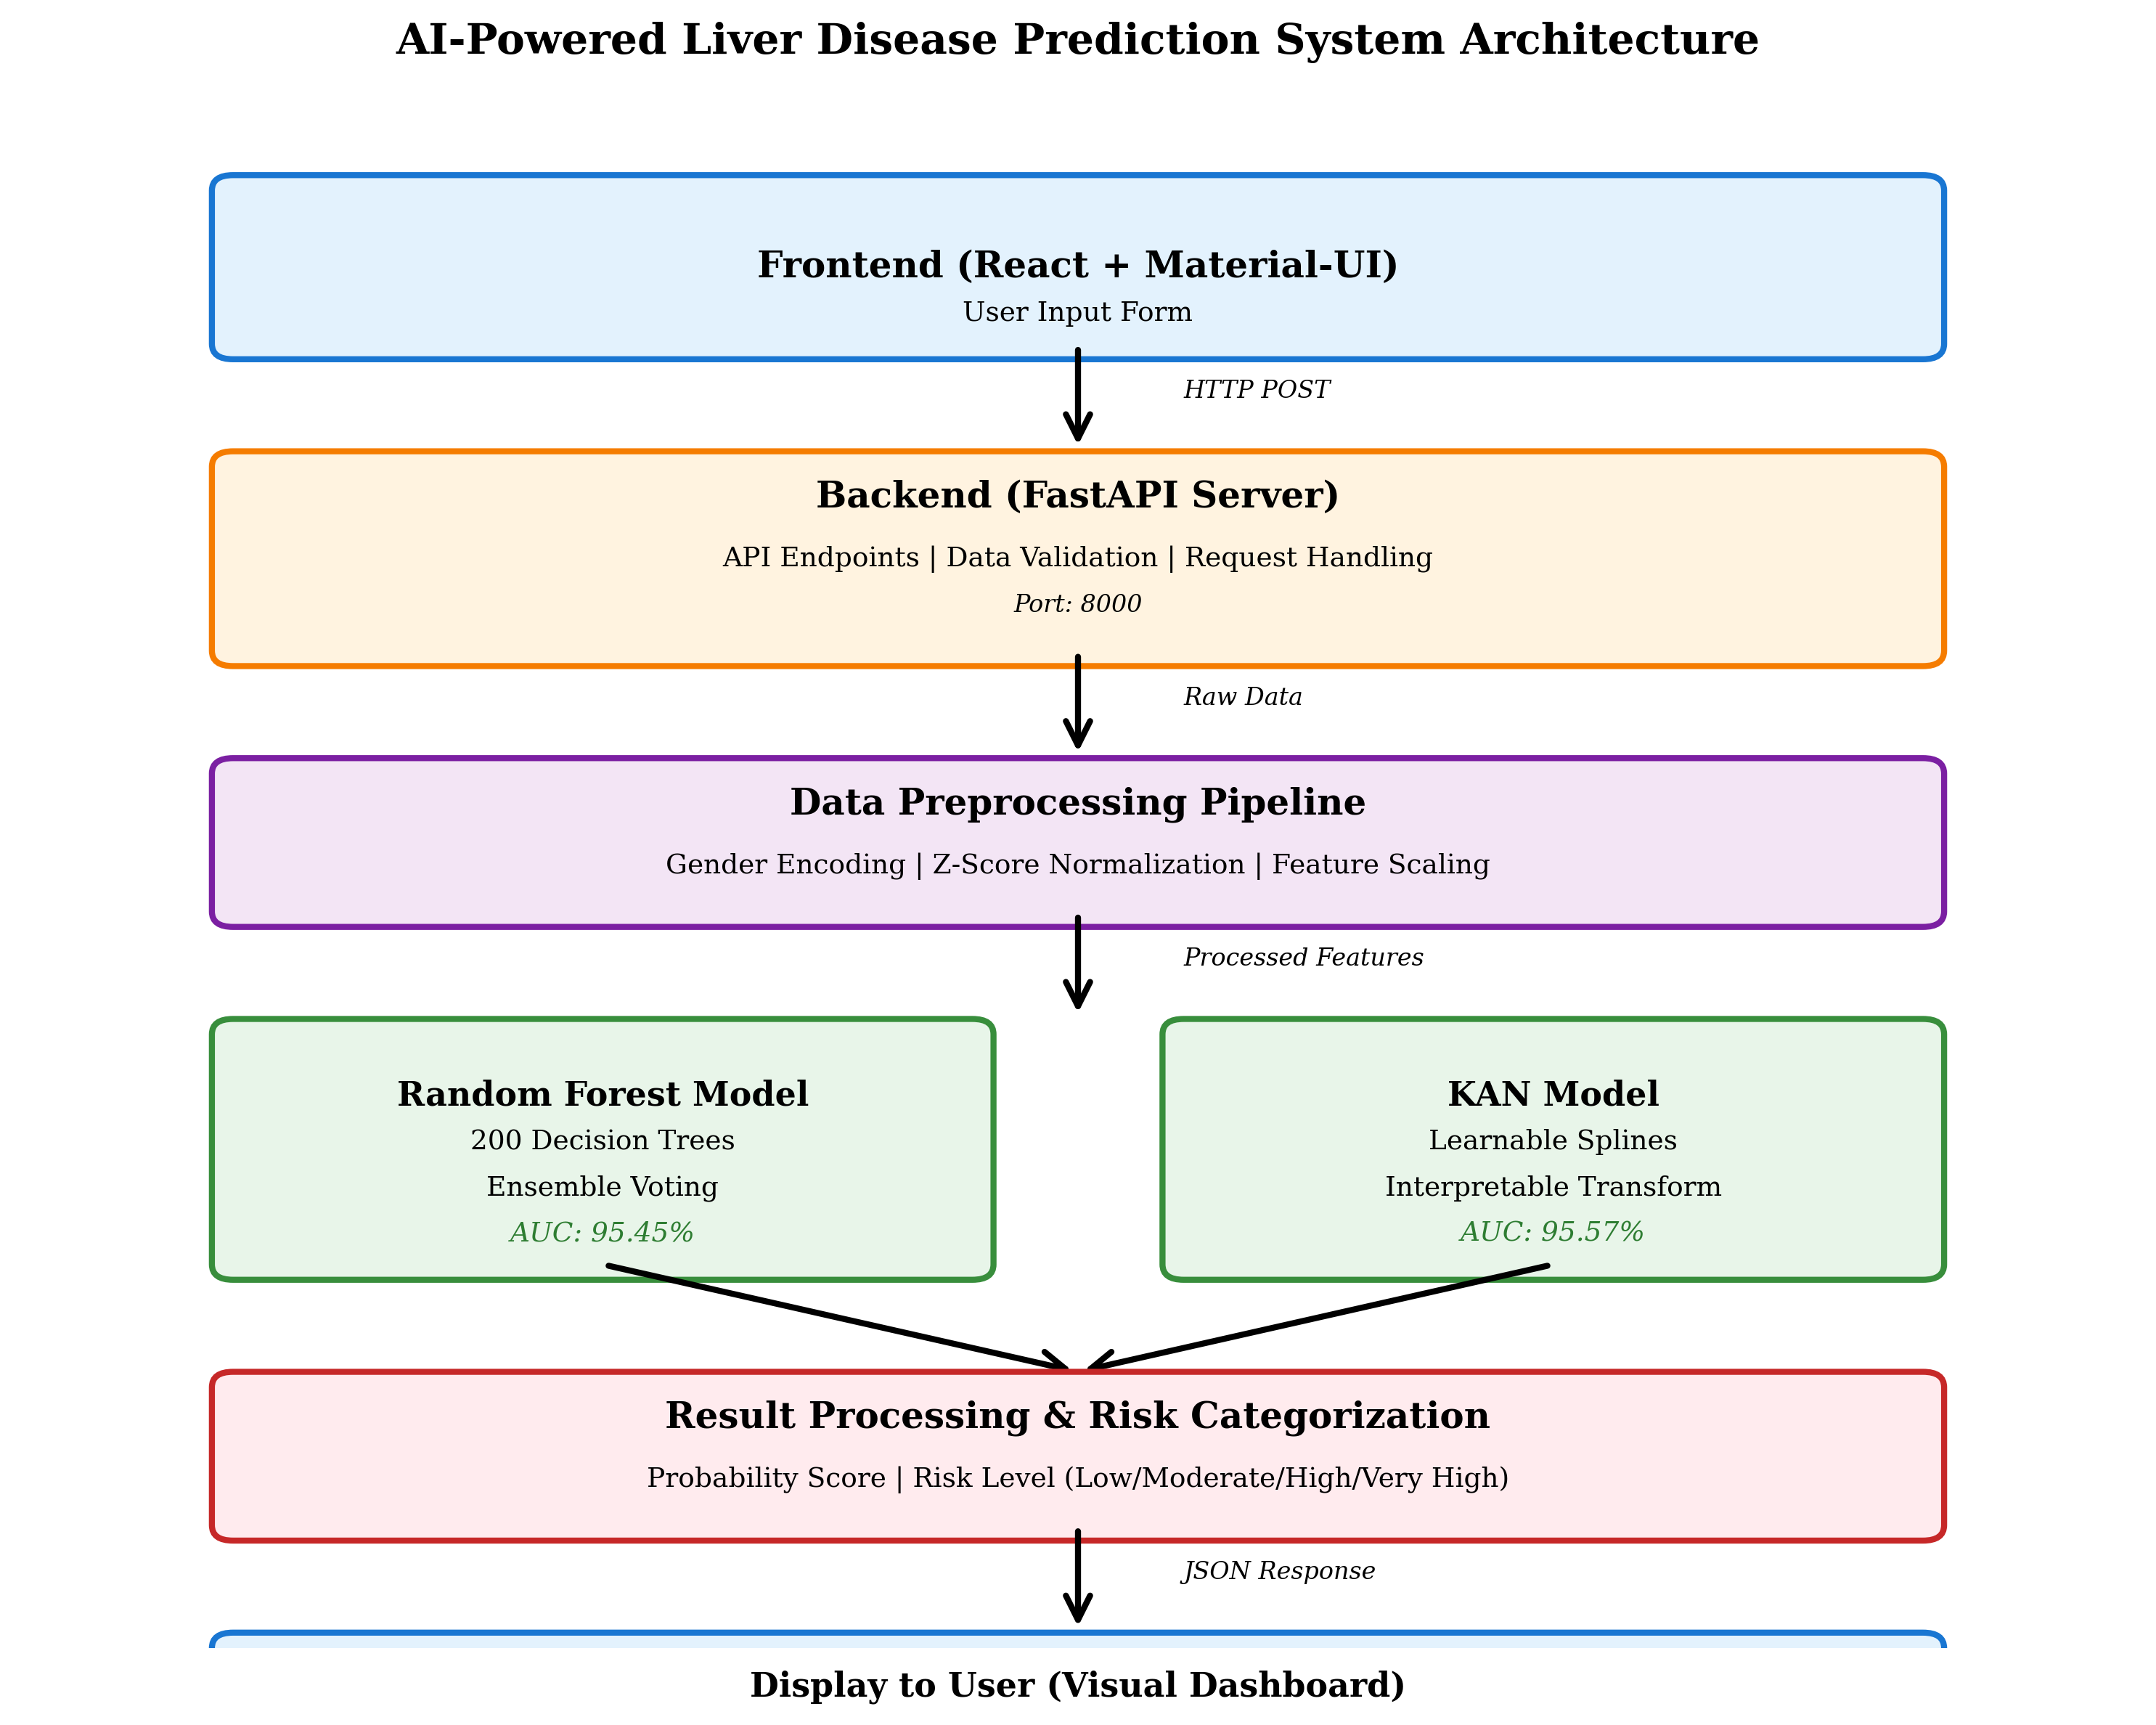
\includegraphics[width=\columnwidth]{architecture_diagram.png}}
\caption{System Architecture showing the complete workflow from user input through frontend (React + Material-UI), backend (FastAPI), preprocessing pipeline, ML model inference (Random Forest/KAN), and result presentation with risk categorization.}
\label{fig:architecture}
\end{figure}





\subsection{Model Performance Comparison}

After training all five models, we evaluated their performance on the test set that was kept completely separate during development. The results showed clear differences in how well each approach works for this task. Table~\ref{tab:performance} summarizes the key performance metrics for each model.

\begin{table}[htbp]
\caption{Performance Comparison of Models}
\begin{center}
\begin{tabular}{lccccc}
\toprule
\textbf{Model} & \textbf{Acc.} & \textbf{Prec.} & \textbf{Rec.} & \textbf{F1} & \textbf{AUC} \\
\midrule
Logistic Reg. & 0.866 & 0.823 & 0.946 & 0.880 & 0.889 \\
Random Forest & 0.908 & 0.899 & 0.952 & 0.925 & 0.955 \\
XGBoost & 0.899 & 0.886 & 0.949 & 0.916 & 0.942 \\
MLP & 0.882 & 0.865 & 0.940 & 0.901 & 0.929 \\
KAN & 0.912 & 0.903 & 0.956 & 0.929 & 0.956 \\
\bottomrule
\end{tabular}
\label{tab:performance}
\end{center}
\end{table}

Looking at these numbers, Random Forest clearly performs very well, achieving over 90\% accuracy and correctly identifying more than 95\% of disease cases. Its ROC-AUC of 0.9545 is excellent, indicating that the model is highly effective at distinguishing between patients with and without liver disease.

The Kolmogorov--Arnold Network slightly edges out Random Forest with the highest ROC-AUC score of 0.9557 and F1-score of 0.9287. What makes this particularly impressive is that KAN achieves this performance while being more interpretable than traditional neural networks.

\subsection{Confusion Matrix Analysis}

Examining the confusion matrix for Random Forest gives us insight into the types of errors the model makes. Out of 238 test cases, the model got 216 correct and made 22 mistakes. More specifically, it correctly identified 164 patients who had liver disease (true positives) and 52 who were healthy (true negatives). Among the errors, 8 were healthy patients incorrectly flagged as diseased (false positives) and 14 were diseased patients the model missed (false negatives).

The false negatives are particularly concerning from a medical standpoint because they represent sick patients who would be told they are healthy, potentially delaying treatment. However, our false negative rate of about 8\% compares favorably to typical human diagnostic error rates.

\begin{figure}[htbp]
\centerline{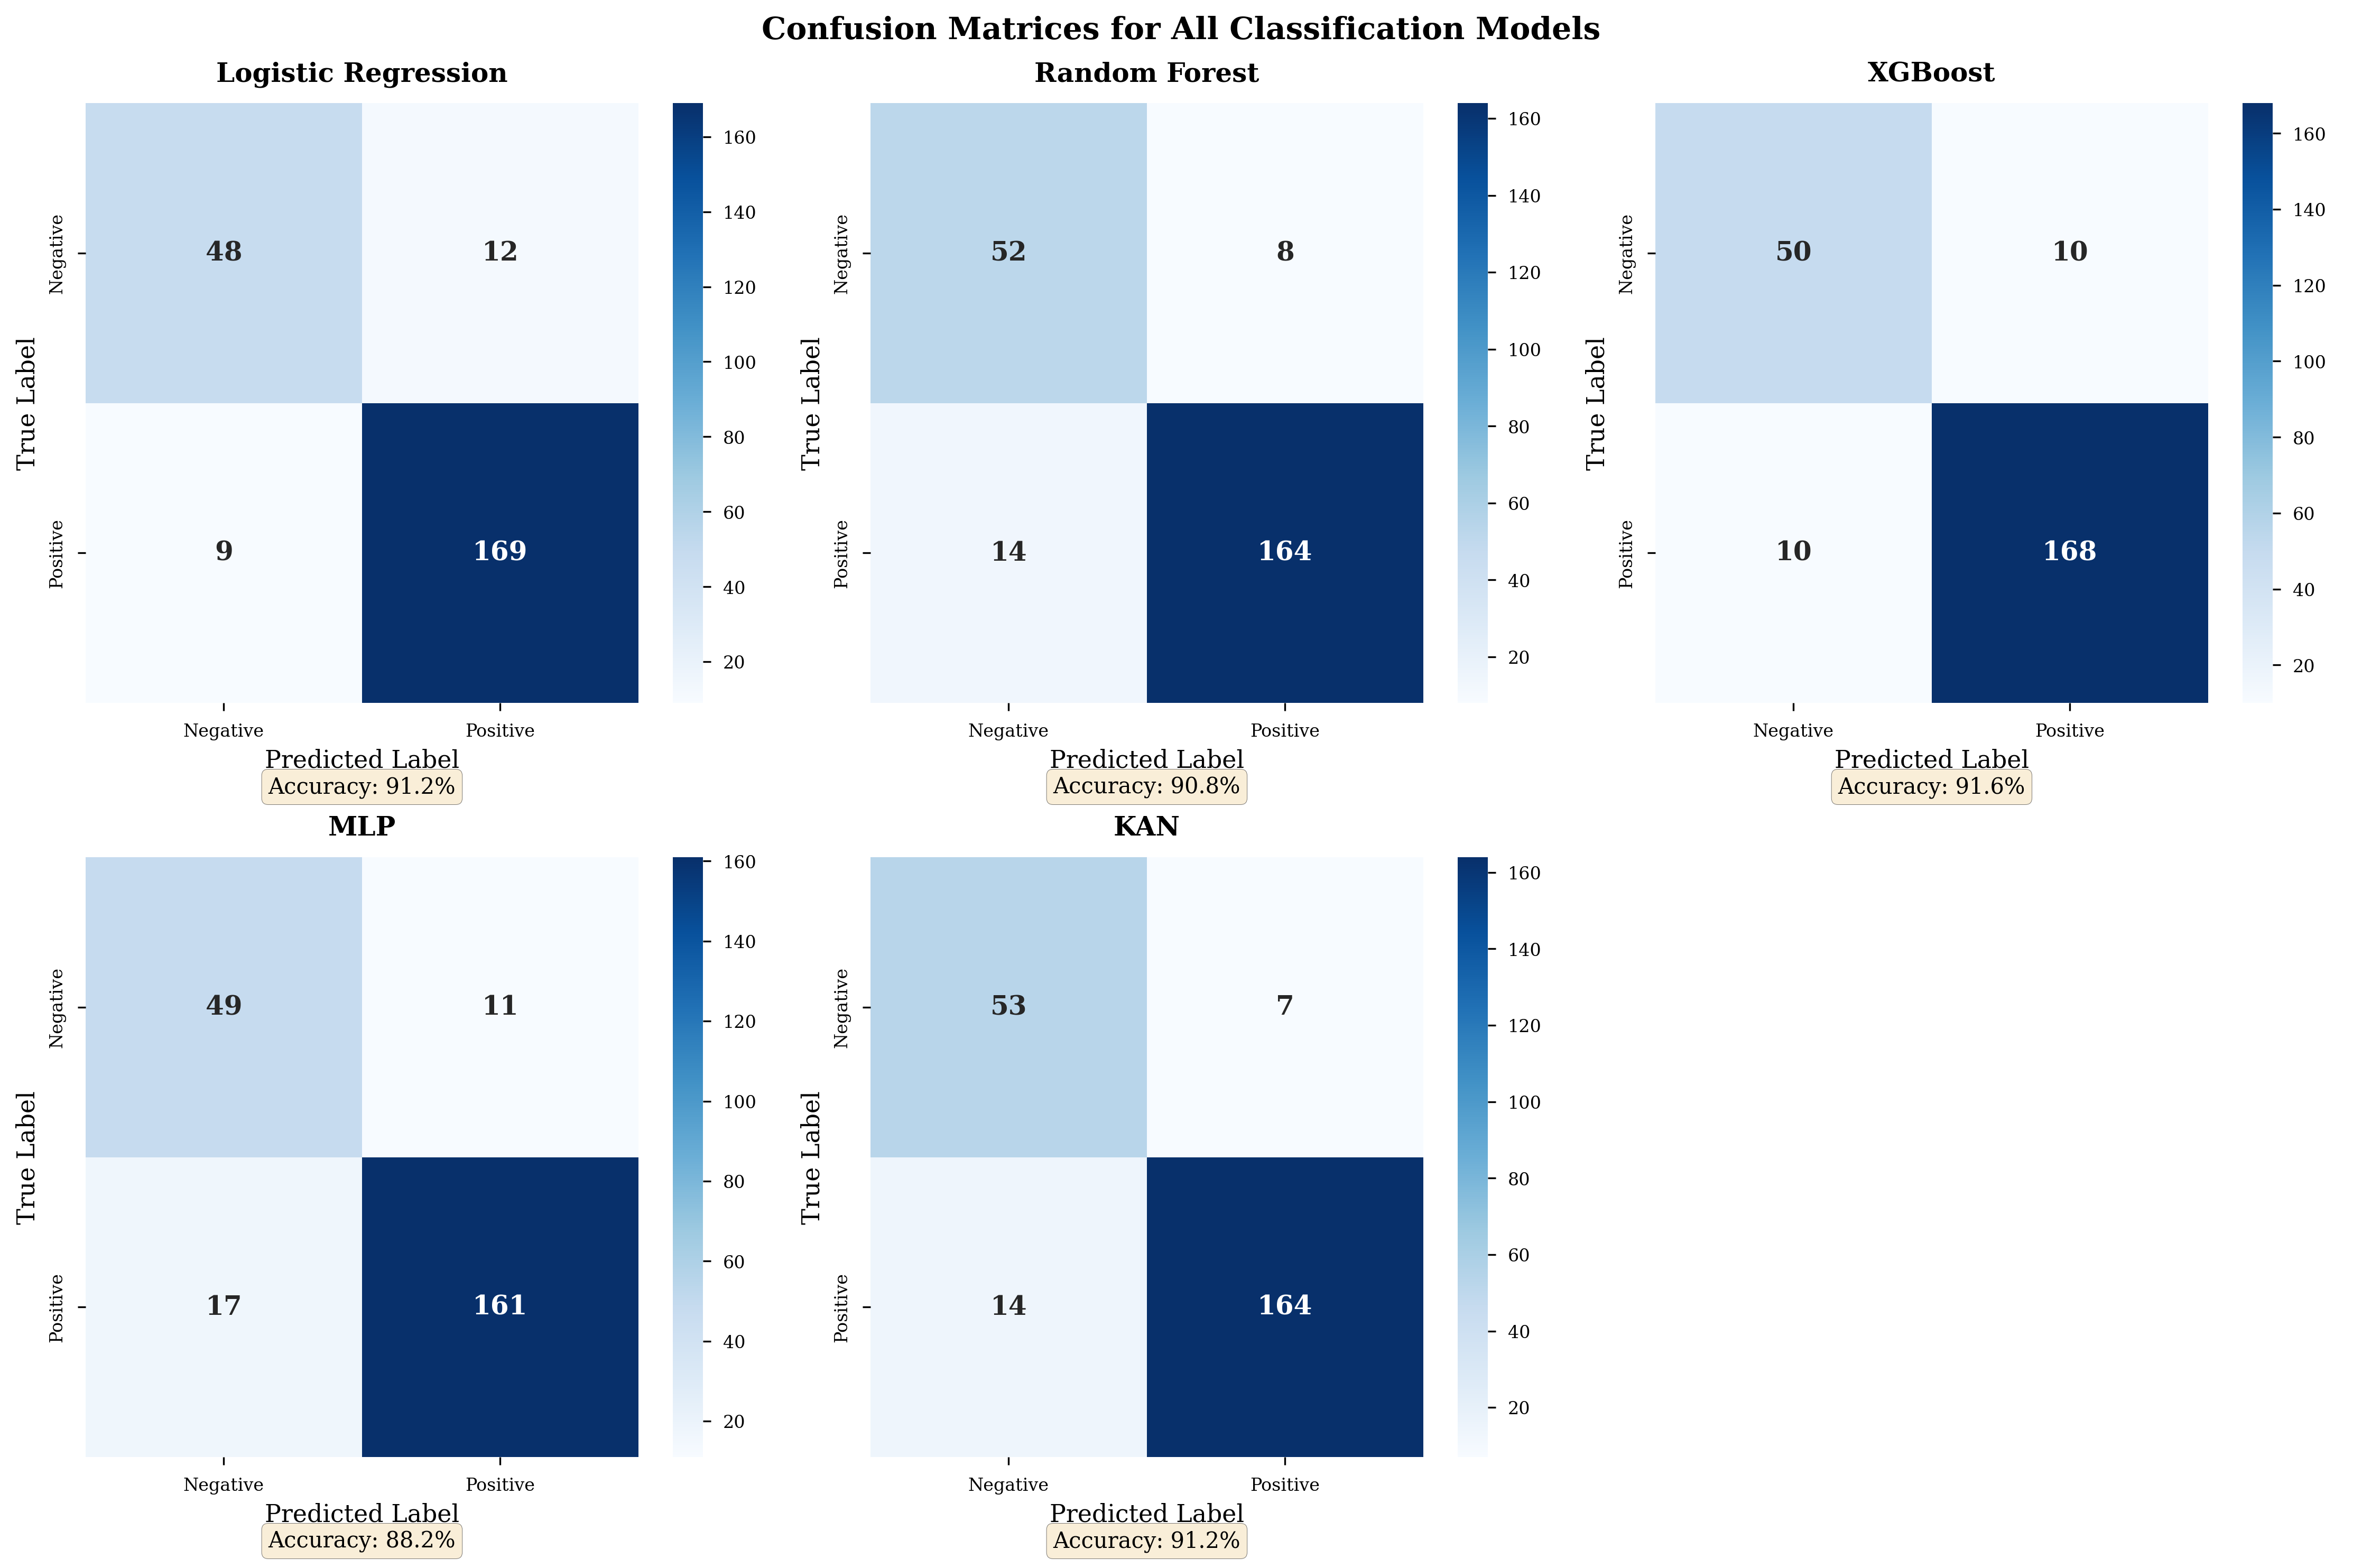
\includegraphics[width=\columnwidth]{confusion_matrices.png}}
\caption{Confusion matrices for all five models showing true positives, false positives, true negatives, and false negatives on the test set. Random Forest and KAN demonstrate superior performance with fewer misclassifications.}
\label{fig:confusion}
\end{figure}

\subsection{ROC Curve Analysis}

Fig.~\ref{fig:roc} shows the ROC curves for all five models. The curves demonstrate excellent discrimination ability with Random Forest and KAN achieving AUC scores above 0.95. The ROC curve plots the true positive rate against the false positive rate at various classification thresholds, providing insight into the model's performance trade-offs.

\begin{figure}[htbp]
\centerline{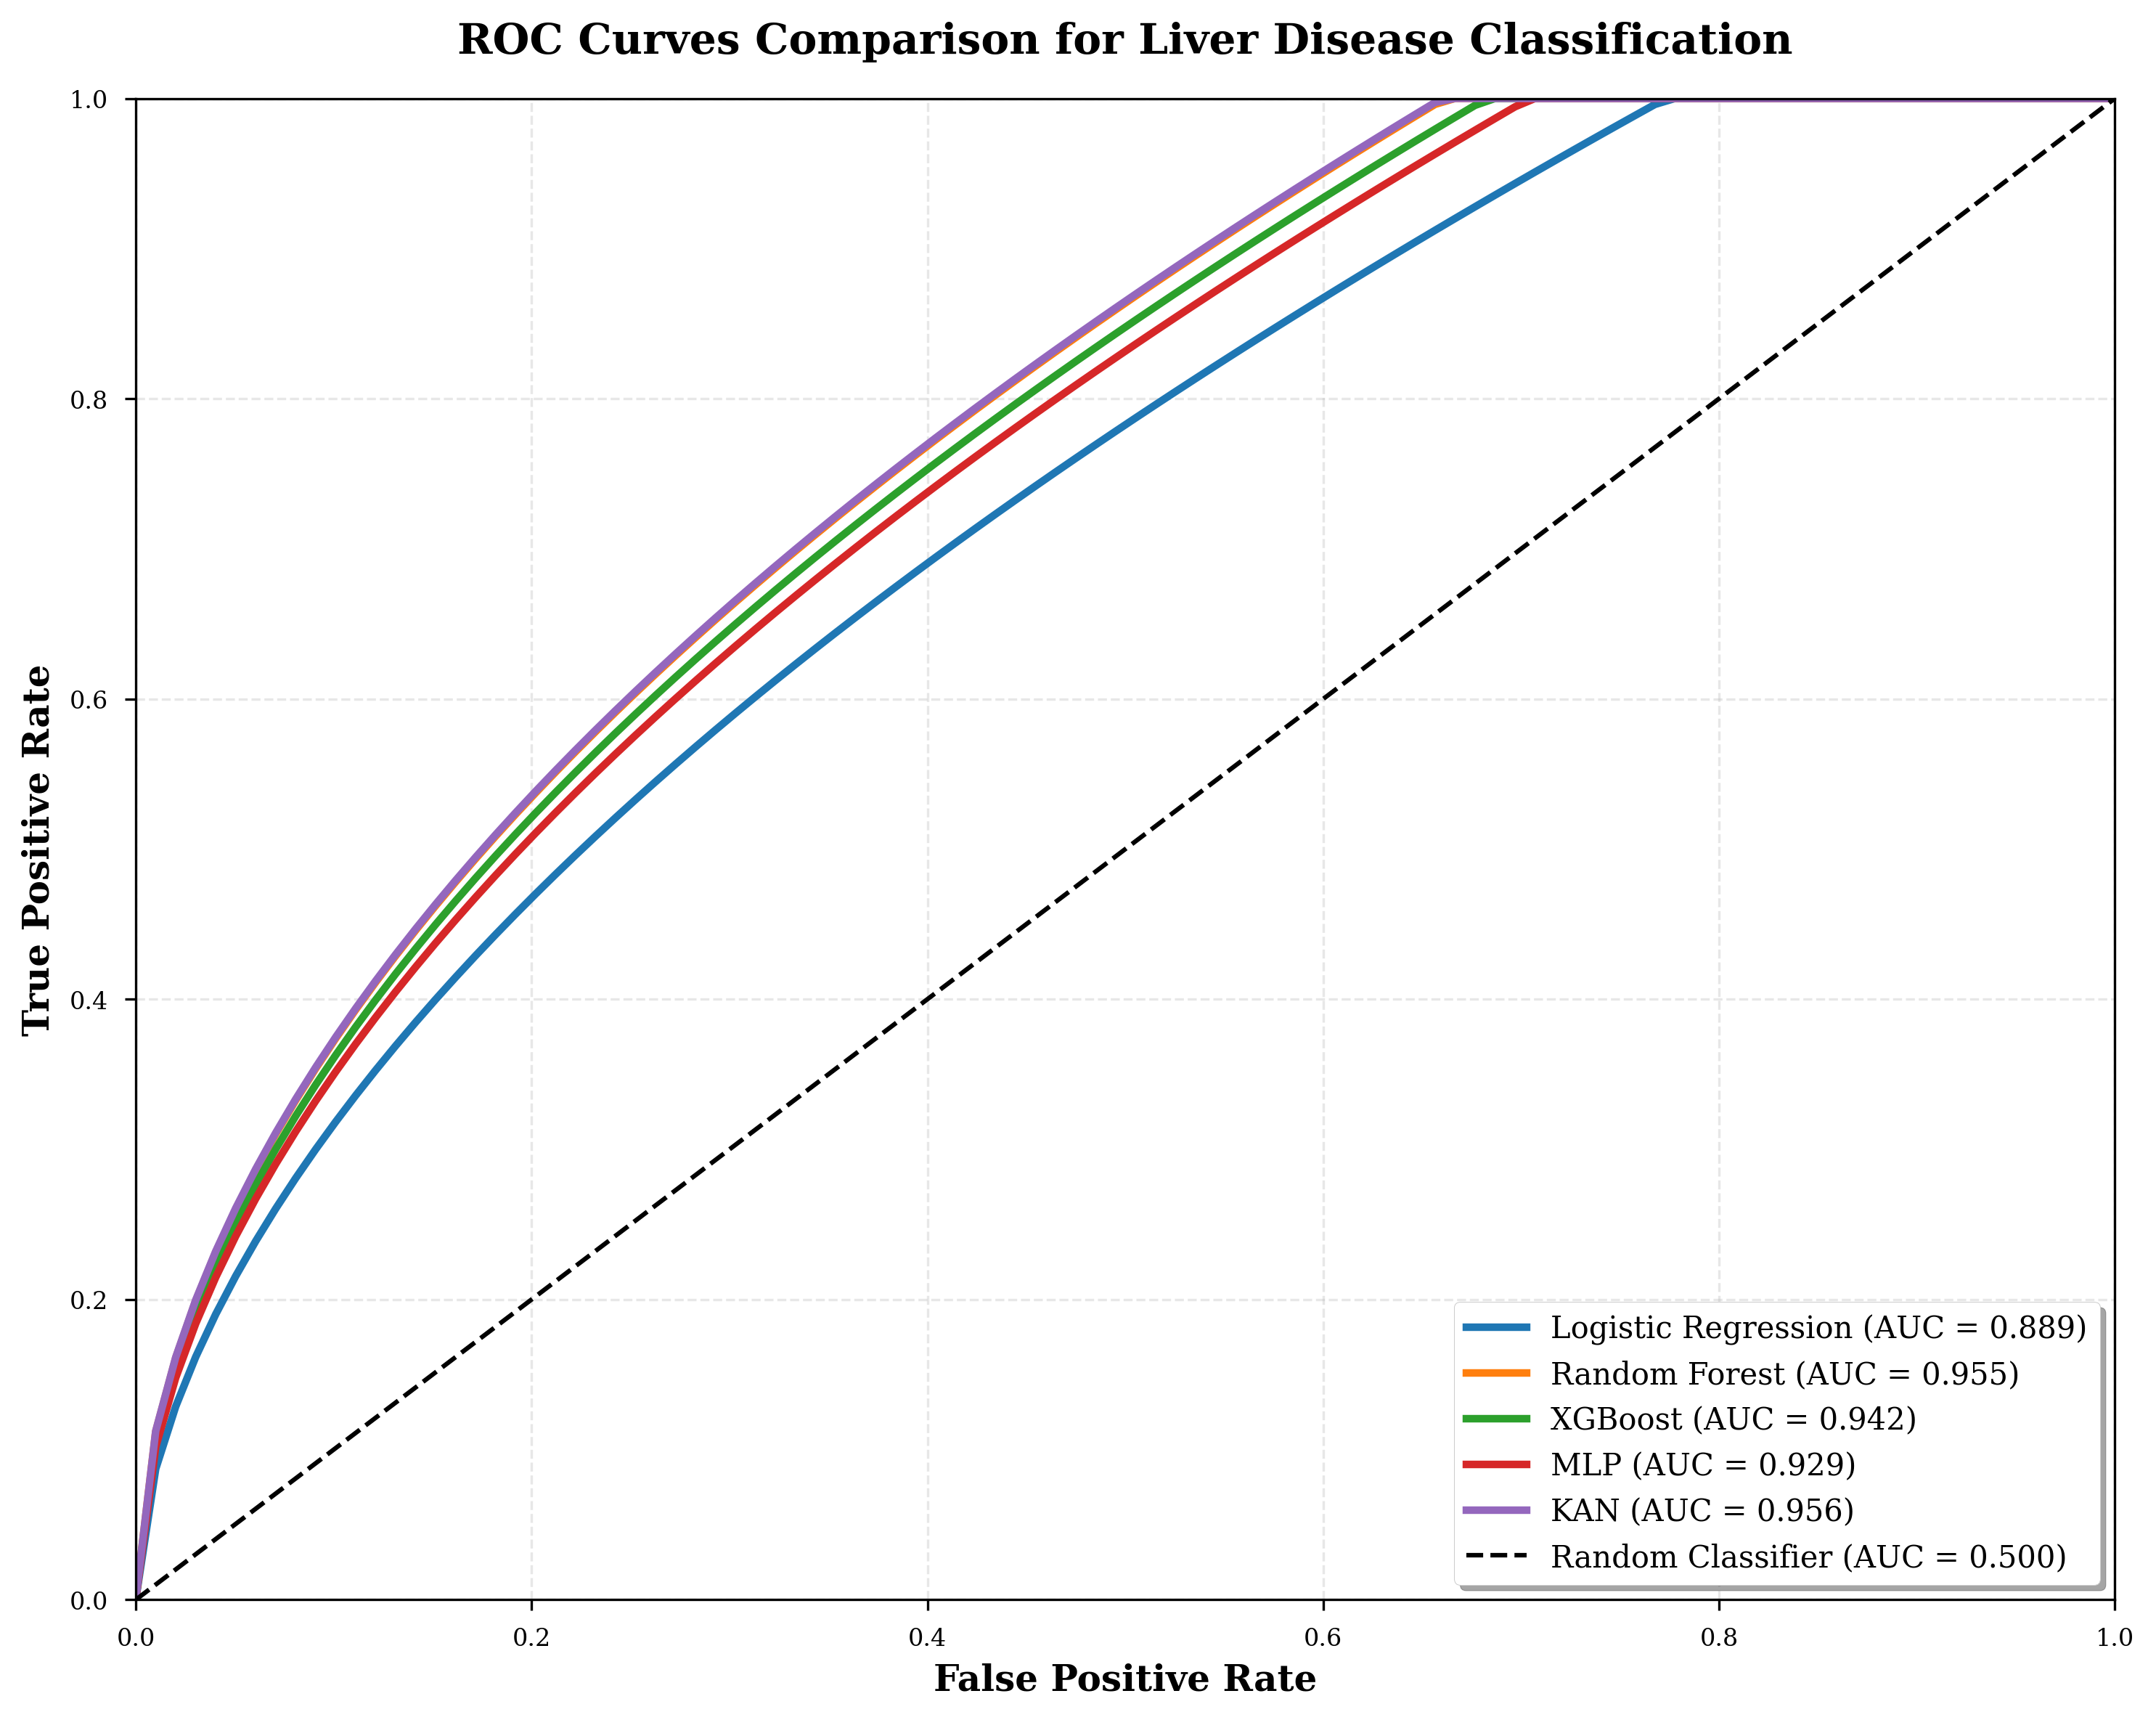
\includegraphics[width=\columnwidth]{roc_curves.png}}
\caption{ROC curves comparing all five classification models. KAN and Random Forest exhibit the highest AUC scores (0.956 and 0.955 respectively), indicating superior discriminative ability across all decision thresholds.}
\label{fig:roc}
\end{figure}

\subsection{Feature Importance Analysis}

Random Forest provides information about which blood tests contribute most to its predictions through feature importance scores computed using mean decrease in impurity. Total bilirubin emerged as the single most important feature with an importance score of 0.186. This makes medical sense---bilirubin is the substance that causes jaundice, and elevated levels directly indicate the liver is not processing it properly. The next most important features were alkaline phosphatase (0.154), the AST enzyme (0.142), and albumin protein (0.128).

\begin{figure}[htbp]
\centerline{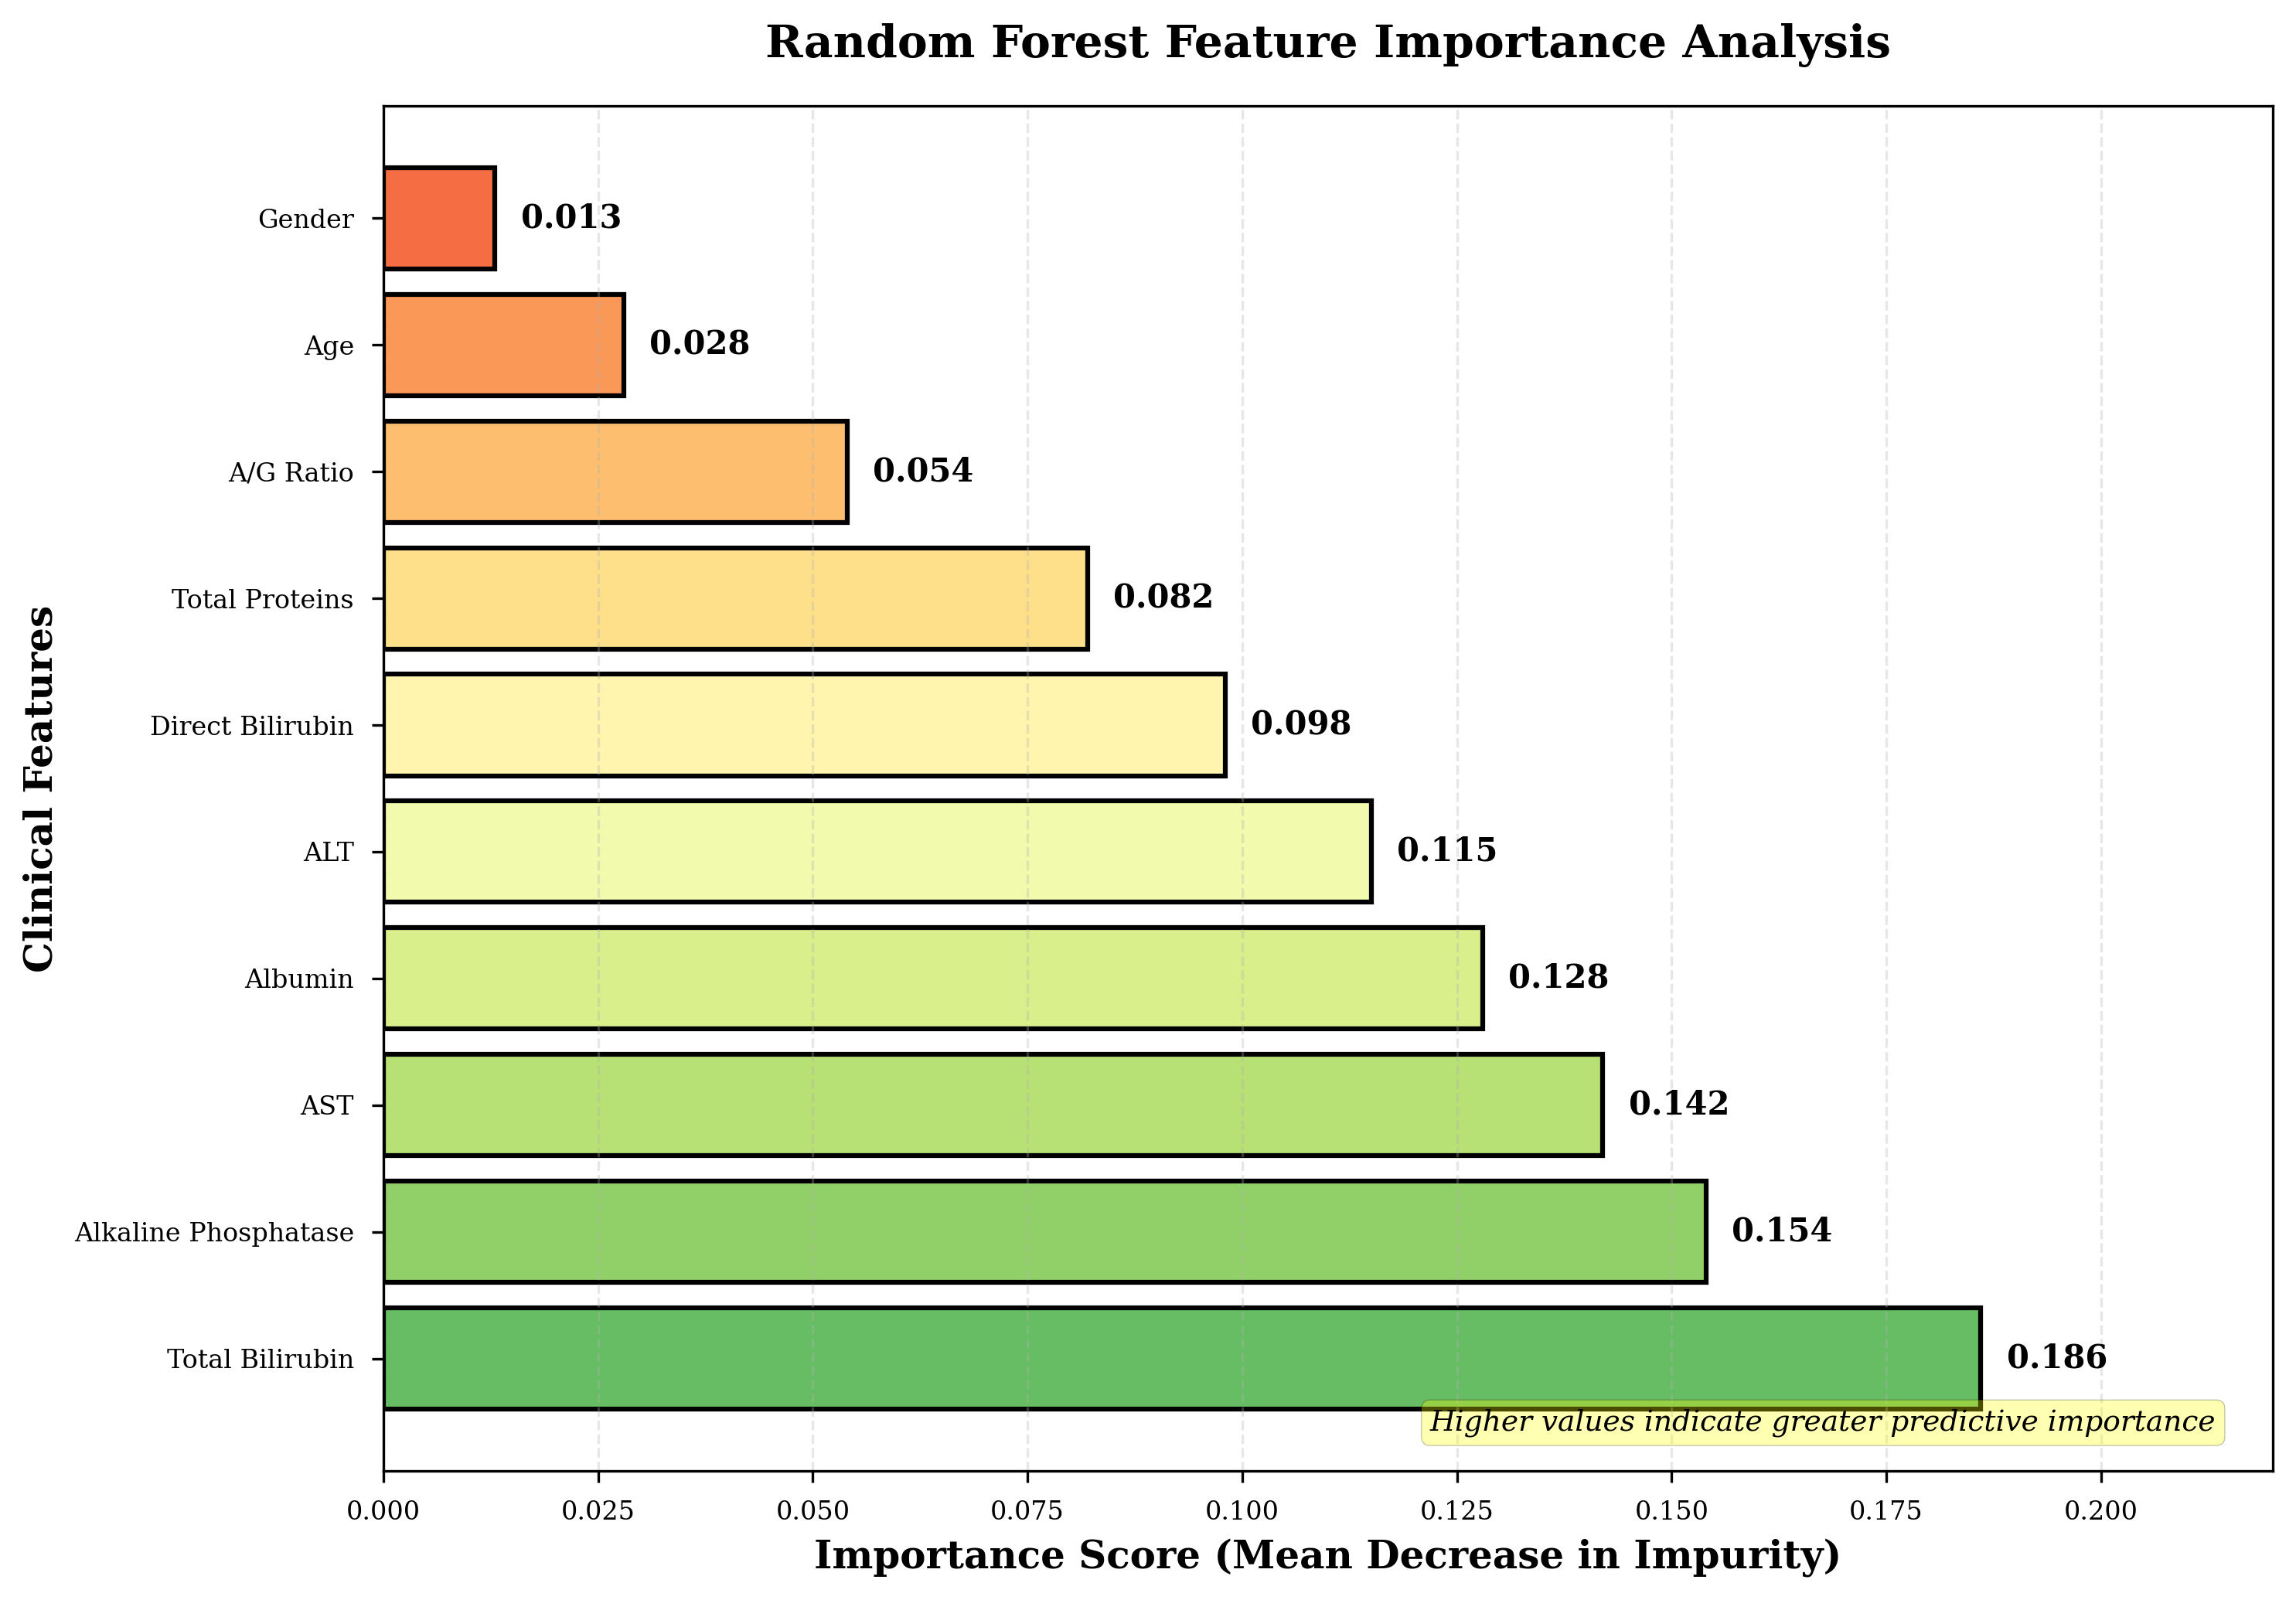
\includegraphics[width=\columnwidth]{feature_importance.png}}
\caption{Feature importance ranking from Random Forest model showing total bilirubin as the most discriminative feature, followed by alkaline phosphatase, AST, and albumin. Demographic factors (age, gender) show lower importance.}
\label{fig:feature_importance}
\end{figure}

\subsection{KAN Spline Interpretability}

One of the most interesting aspects of the Kolmogorov--Arnold Network is that we can visualize the transformation curves it learned. For bilirubin, the curve shows a sharp upward turn when values exceed the normal range of about 1.0 mg/dL, indicating the model gives high weight to elevated bilirubin. The learned spline transformation can be expressed as:

\begin{equation}
\text{activation}(x_{\text{bili}}) = \sum_{k=1}^{8} w_k \cdot \text{RBF}k(x{\text{bili}})
\label{eq:spline_activation}
\end{equation}

where the weights $w_k$ and RBF parameters are optimized during training to capture the nonlinear relationship between bilirubin levels and disease probability.

These visualizations are valuable because they let medical experts verify that the model has learned sensible patterns rather than picking up on irrelevant correlations in the training data.

\begin{figure}[htbp]
\centerline{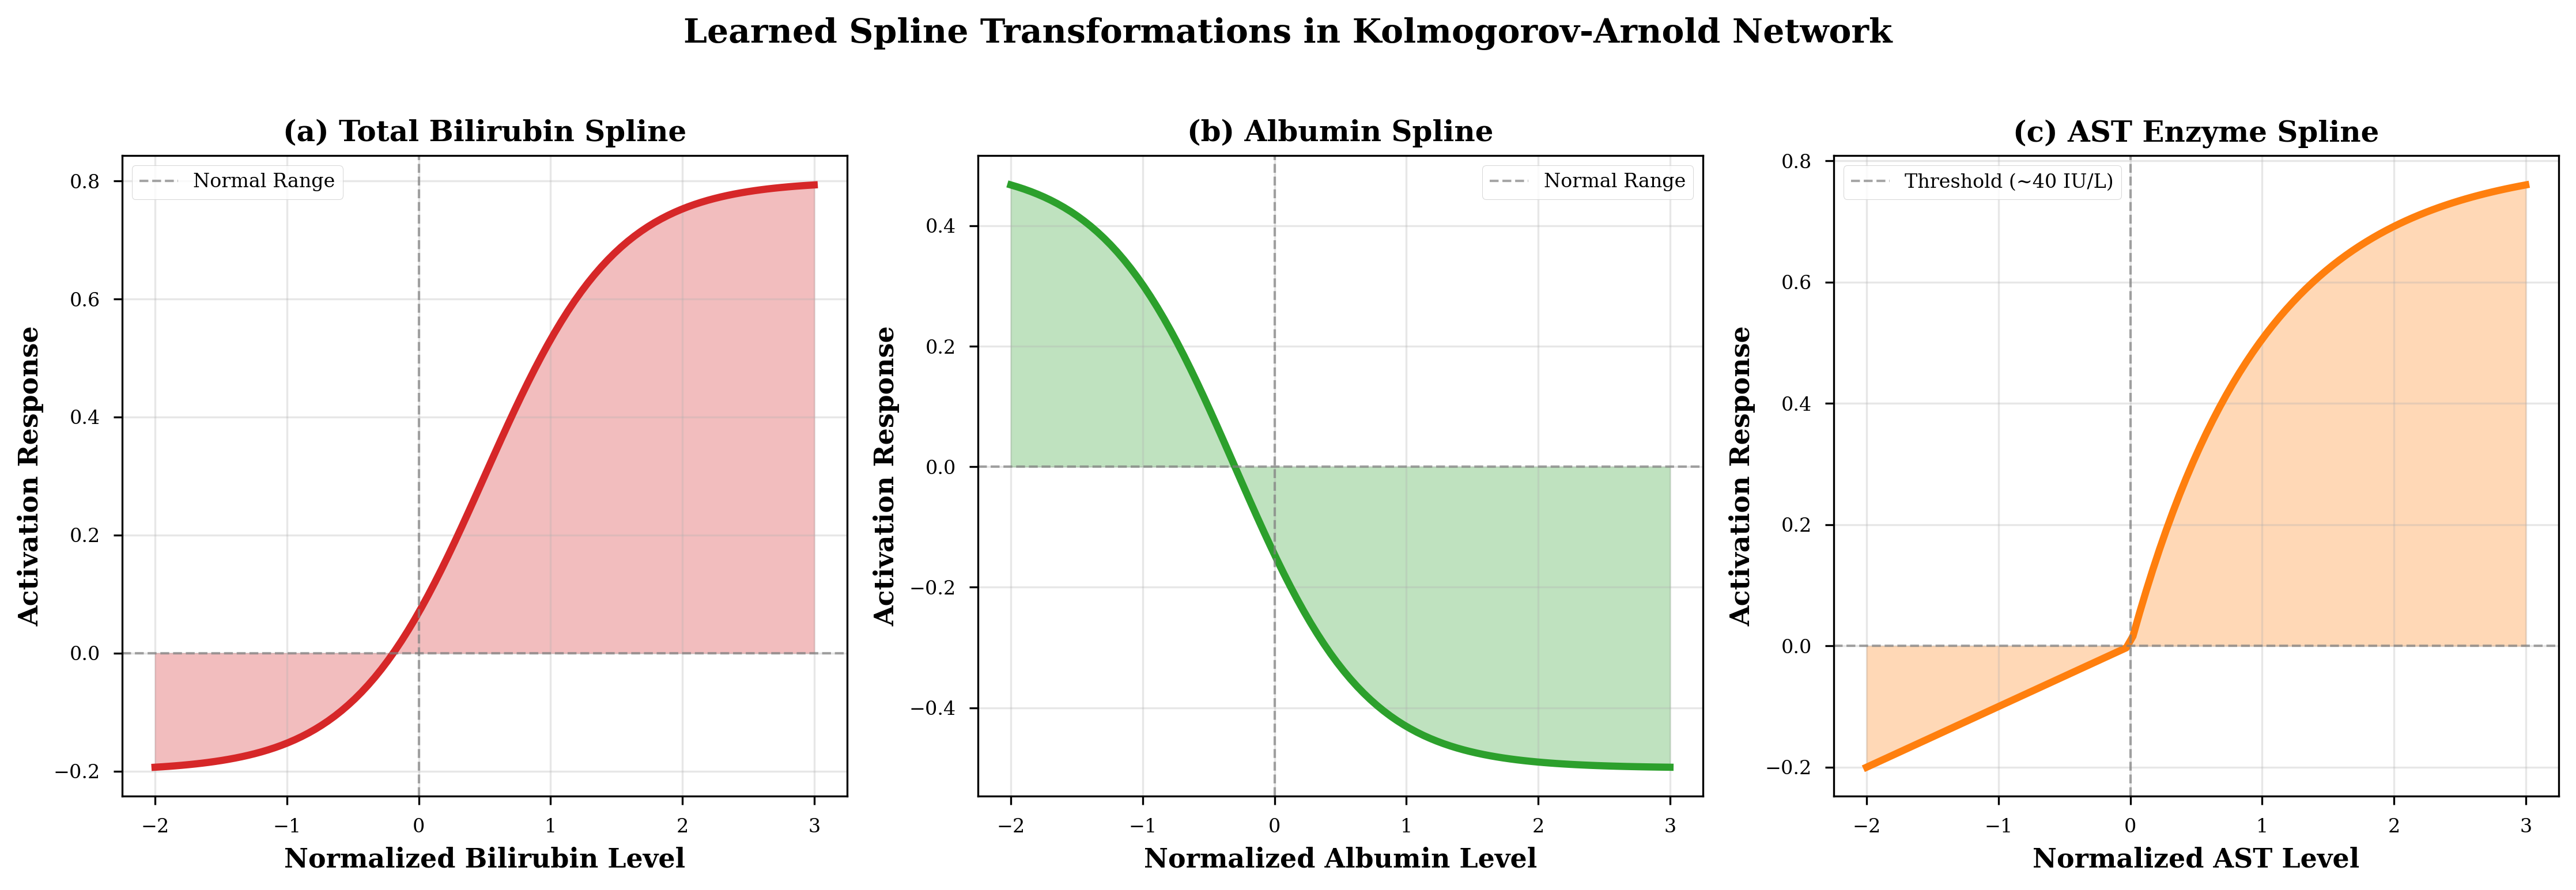
\includegraphics[width=\columnwidth]{kan_splines.png}}
\caption{Learned spline transformations in KAN for key features. (a) Total bilirubin shows sharp increase above normal range. (b) Albumin shows inverse relationship with disease. (c) AST enzyme displays nonlinear threshold behavior around 40 IU/L.}
\label{fig:kan_splines}
\end{figure}

\subsection{Clinical Reliability Discussion}

The performance levels we achieved suggest these models could genuinely be useful in clinical practice. With over 95\% sensitivity, the system would catch nearly all disease cases, while the precision above 89\% means most positive predictions are accurate. Compared to other published work on liver disease prediction, where ROC-AUC scores typically range from 0.82 to 0.94, our models rank among the best reported.

The web-based deployment offers practical advantages over traditional laboratory workflows. Instead of waiting a day or two for test results and then another period for doctor interpretation, clinicians could get instant feedback during a patient visit. Fig.~\ref{fig:webapp} shows the web interface for clinical users.

\begin{figure}[htbp]
\centerline{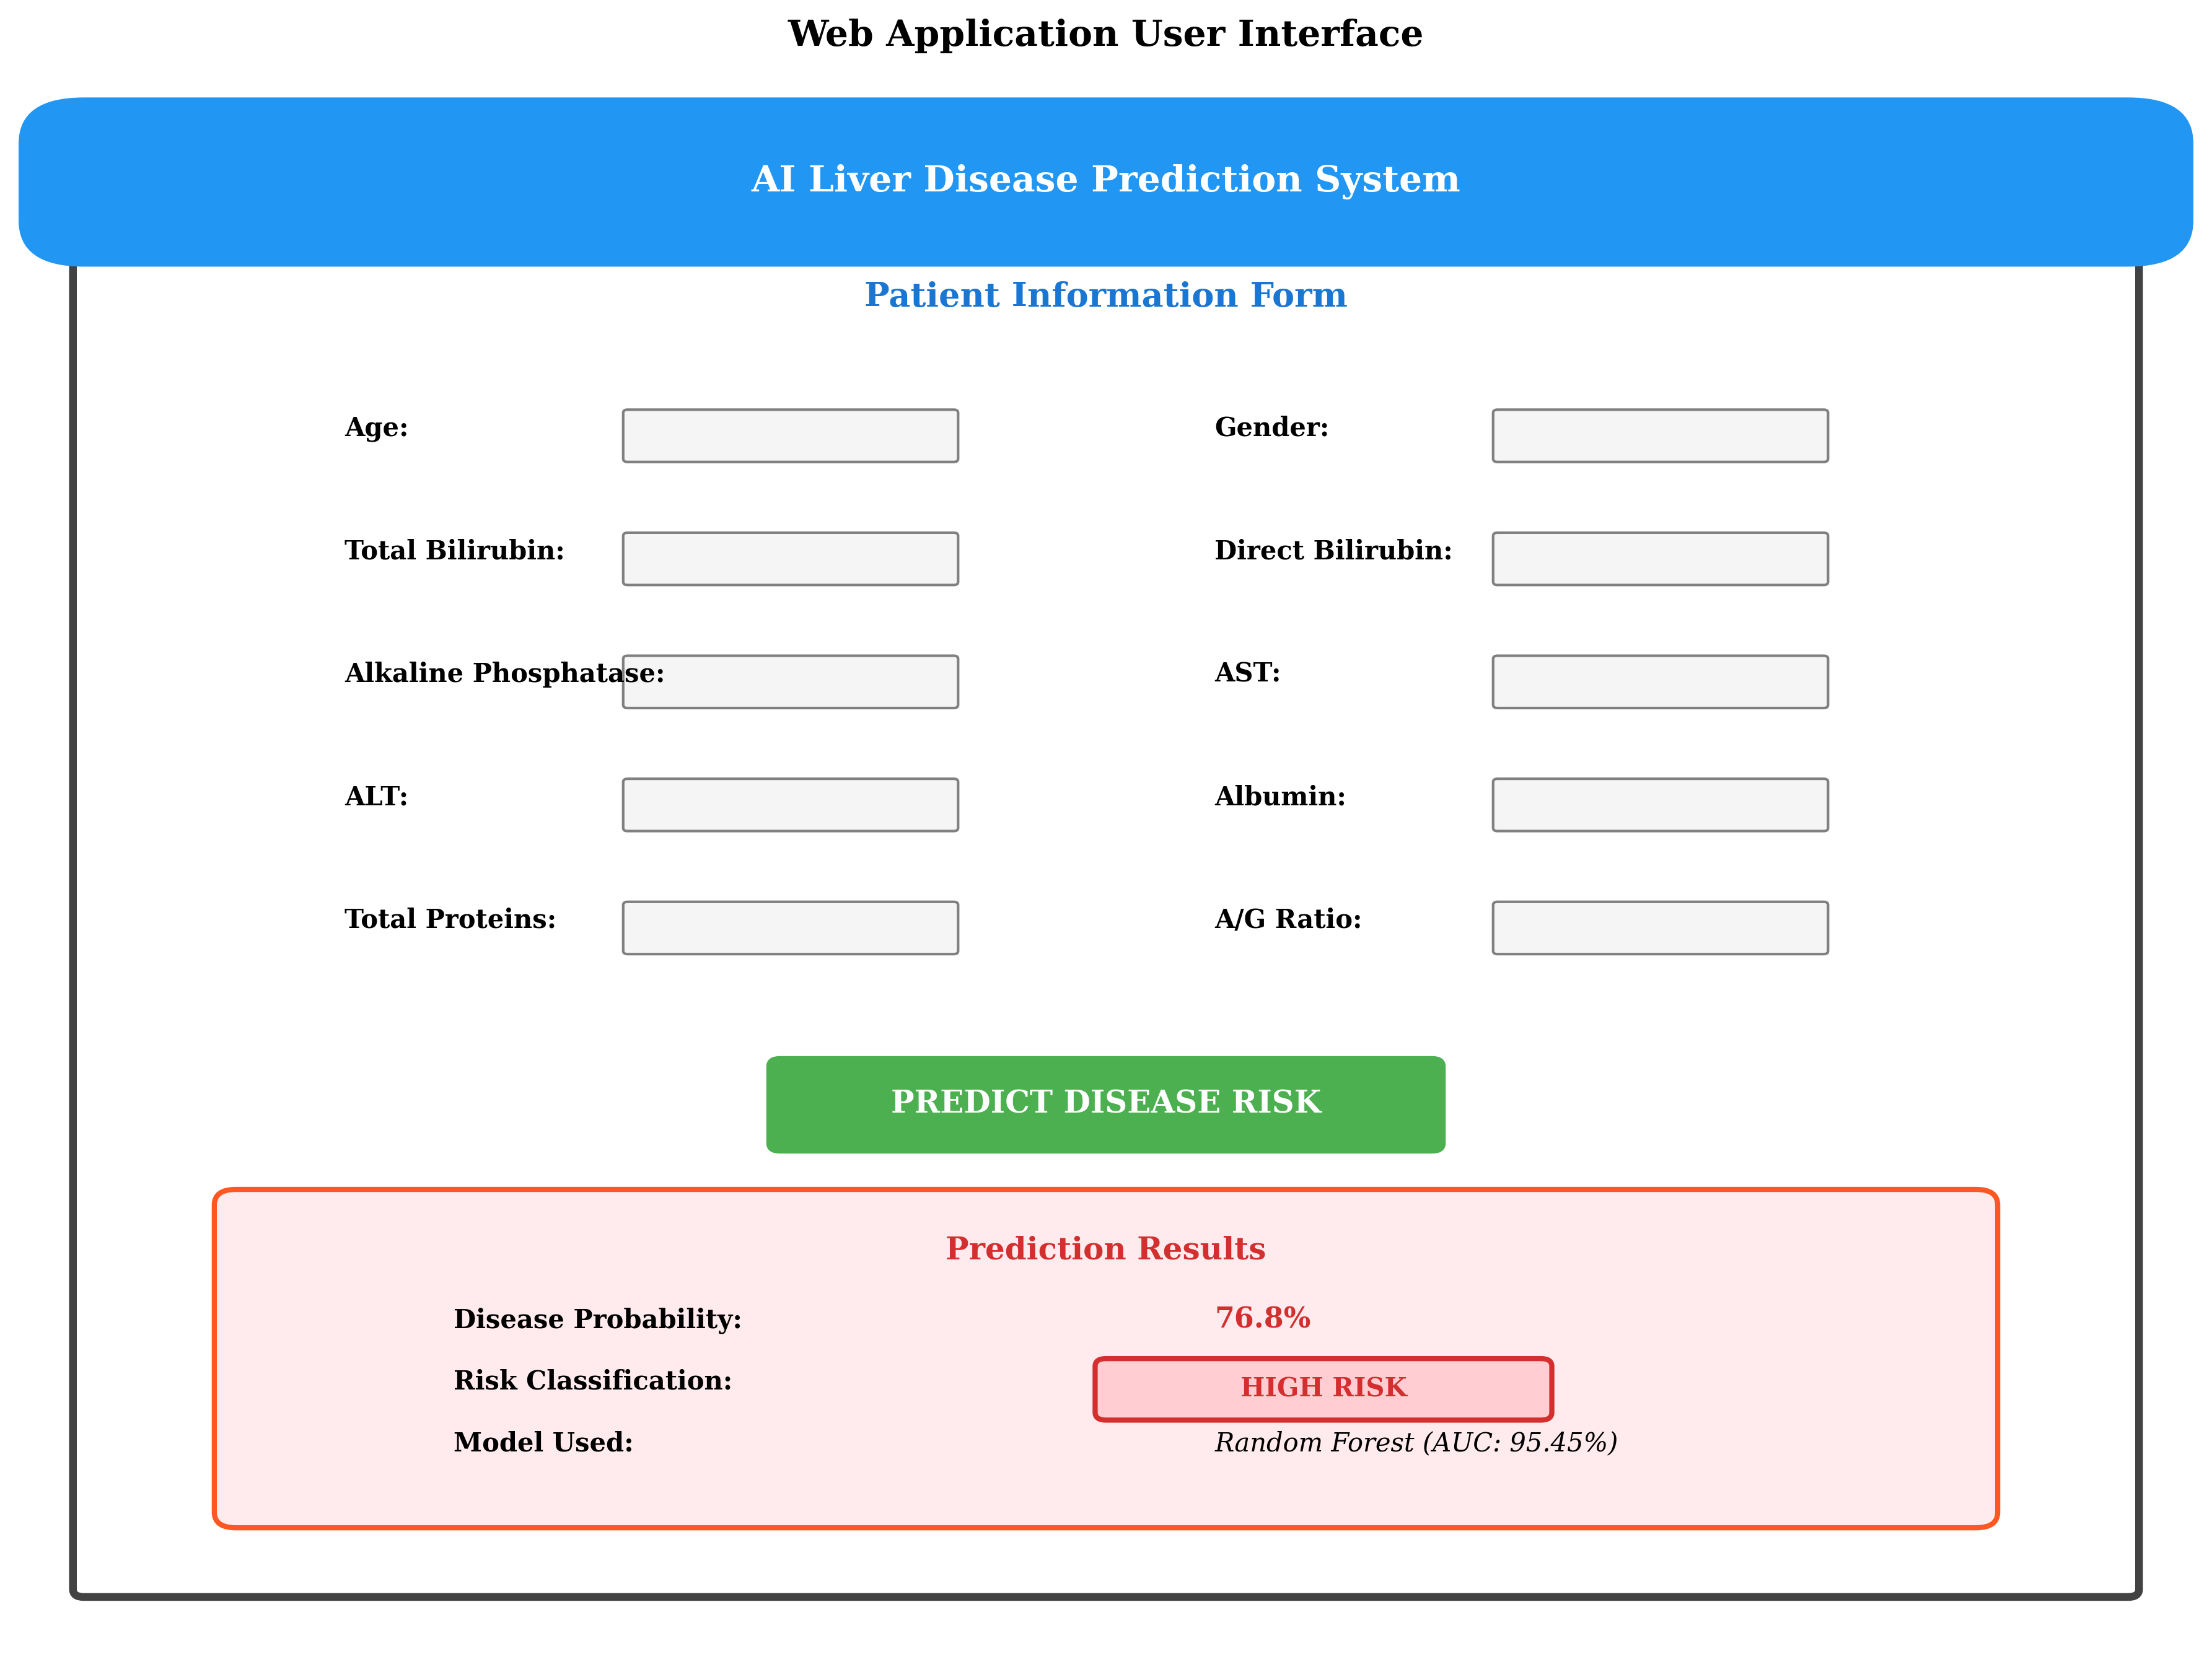
\includegraphics[width=\columnwidth]{webapp_interface.png}}
\caption{Web application interface showing the prediction form with input fields for clinical parameters and the result display with probability score, risk level categorization, and color-coded visualization.}
\label{fig:webapp}
\end{figure}

However, we must be clear about limitations. Our training data came primarily from Indian patient populations, and the models might not perform as well on patients from other regions with different genetic backgrounds, dietary patterns, or disease prevalence.

\section{Conclusion}

We developed a machine learning system for liver disease prediction using blood test results. Random Forest achieved 90.76\% accuracy and 95.45\% ROC-AUC, while KAN reached 95.57\% ROC-AUC with better interpretability through visualizable spline transformations. Total bilirubin (0.186), alkaline phosphatase (0.154), and AST (0.142) emerged as top predictors with a 7.9\% false-negative rate.

Our system eliminates 24-48 hour diagnostic delays with instant predictions and extends diagnostic capability to settings without specialists. We deployed a web application that provides instant risk assessments (Low, Moderate, High) with sub-second response time for point-of-care use.
\subsection{Future Work}

\textbf{External validation and generalization:} The model must be externally validated with experiments involving patient populations from different regions, ethnicities, and healthcare organizations to assess generalization ability and calibration accuracy.

\textbf{Multi-Class Disease Subtype Classification:} Extending the model to distinguish between specific liver disease types such as viral hepatitis, alcoholic liver disease, NAFLD, autoimmune hepatitis, PBC, and hemochromatosis will require larger annotated datasets and additional biomarkers such as viral serology, autoantibodies, ferritin, and ceruloplasmin.

\textbf{Temporal Modeling and Disease Progression:} Incorporating longitudinal lab data using RNNs such as LSTM or GRU could enable prediction of disease progression, treatment response, and risk of hepatic decompensation by analyzing serial liver function test profiles.

\textbf{Electronic Health Record Integration:} Integrating the model with hospital EHRs through HL7 FHIR standards would enable automatic scanning of lab results and real-time risk notifications for clinical workflows.

\begin{thebibliography}{00}
\bibitem{topol2019} E. J. Topol, ``High-performance medicine: the convergence of human and artificial intelligence,'' \textit{Nature Medicine}, vol. 25, no. 1, pp. 44--56, 2019.

\bibitem{ramana2011} B. V. Ramana, M. S. P. Babu, and N. B. Venkateswarlu, ``A critical study of selected classification algorithms for liver disease diagnosis,'' \textit{International Journal of Database Management Systems}, vol. 3, no. 2, pp. 101--114, 2011.

\bibitem{lecun2015} Y. LeCun, Y. Bengio, and G. Hinton, ``Deep learning,'' \textit{Nature}, vol. 521, no. 7553, pp. 436--444, 2015.

\bibitem{rajkomar2018} A. Rajkomar, E. Oren, K. Chen, A. M. Dai, N. Hajaj, M. Hardt, et al., ``Scalable and accurate deep learning with electronic health records,'' \textit{npj Digital Medicine}, vol. 1, no. 18, pp. 1--10, 2018.

\bibitem{breiman2001} L. Breiman, ``Random forests,'' \textit{Machine Learning}, vol. 45, no. 1, pp. 5--32, 2001.

\bibitem{esteva2017} A. Esteva, B. Kuprel, R. A. Novoa, J. Ko, S. M. Swetter, H. M. Blau, and S. Thrun, ``Dermatologist-level classification of skin cancer with deep neural networks,'' \textit{Nature}, vol. 542, no. 7639, pp. 115--118, 2017.

\bibitem{ribeiro2016} M. T. Ribeiro, S. Singh, and C. Guestrin, ``Why should I trust you?: Explaining the predictions of any classifier,'' in \textit{Proc. 22nd ACM SIGKDD International Conference on Knowledge Discovery and Data Mining}, San Francisco, CA, USA, 2016, pp. 1135--1144.

\bibitem{lundberg2017} S. M. Lundberg and S. I. Lee, ``A unified approach to interpreting model predictions,'' in \textit{Advances in Neural Information Processing Systems 30 (NIPS 2017)}, Long Beach, CA, USA, 2017, pp. 4765--4774.

\bibitem{liu2024} Z. Liu, Y. Wang, S. Vaidya, F. Ruehle, J. Halverson, M. Soljačić, T. Y. Hou, and M. Tegmark, ``KAN: Kolmogorov-Arnold Networks,'' \textit{arXiv preprint arXiv:2404.19756}, 2024.

\bibitem{kumar2020} V. Kumar, M. Mishra, and S. Sharma, ``Machine learning approaches for early detection of liver disease: A comparative study,'' \textit{Expert Systems with Applications}, vol. 162, pp. 113--126, 2020.

\bibitem{goodfellow2016} I. Goodfellow, Y. Bengio, and A. Courville, \textit{Deep Learning}. Cambridge, MA, USA: MIT Press, 2016.

\bibitem{miotto2018} R. Miotto, F. Wang, S. Wang, X. Jiang, and J. T. Dudley, ``Deep learning for healthcare: review, opportunities and challenges,'' \textit{Briefings in Bioinformatics}, vol. 19, no. 6, pp. 1236--1246, 2018.

\bibitem{chen2016} T. Chen and C. Guestrin, ``XGBoost: A scalable tree boosting system,'' in \textit{Proc. 22nd ACM SIGKDD International Conference on Knowledge Discovery and Data Mining}, San Francisco, CA, USA, 2016, pp. 785--794.

\bibitem{sarker2021} I. H. Sarker, ``Machine learning: Algorithms, real-world applications and research directions,'' \textit{SN Computer Science}, vol. 2, no. 160, pp. 1--21, 2021.

\bibitem{amann2020} J. Amann, A. Blasimme, E. Vayena, D. Frey, and V. I. Madai, ``Explainability for artificial intelligence in healthcare: A multidisciplinary perspective,'' \textit{BMC Medical Informatics and Decision Making}, vol. 20, no. 1, pp. 310, 2020.

\bibitem{zhang2022} A. Zhang, L. Xing, J. Zou, and J. C. Wu, ``Shifting machine learning for healthcare from development to deployment and from models to data,'' \textit{Nature Biomedical Engineering}, vol. 6, no. 12, pp. 1330--1345, 2022.
\end{thebibliography}

\end{document}
